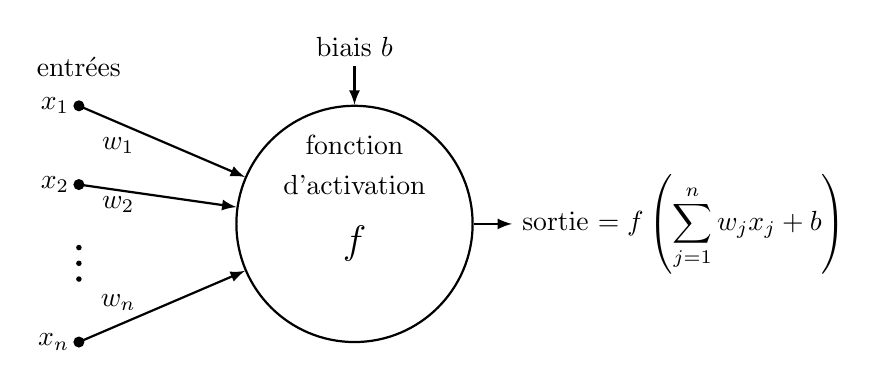
\begin{tikzpicture}

\node [draw, thick, circle, minimum size = 3 cm] (N) at (0,0) {};

\foreach \yi/\N in {1.5/1,0.5/2,-1.5/n}{
\fill (-3.5,\yi) circle(2pt) node [left] {$x_{\N}$};
\draw [thick, -latex] (-3.5,\yi) -- (N);
}

\draw (-3.5,1.75) node [above] {entrées};

\draw (-3,1) node {$w_1$};
\draw (-3,0.25) node {$w_2$};
\draw (-3,-1) node {$w_n$};

\foreach \x/\y in {-3.5/-.5}{
\fill (\x,\y) circle (1pt);
\fill (\x,\y+.2) circle (1pt);
\fill (\x,\y-.2) circle (1pt);
}

\draw [thick, latex-] (N) -- (0,2) node [above] {biais $b$};

\draw [thick, -latex] (N) -- (2,0) node (output) [right] {sortie $\displaystyle = f\left(\sum_{j=1}^n w_jx_j + b\right)$};

\draw (0,-.25) node {\Large $f$};
\draw (0,1) node {fonction};
\draw (0,.5) node {d'activation};

\end{tikzpicture}
